% !TEX root = 0_main.tex
\section{Teilaufgabe 1}
\begin{aufgabe}%1
	\begin{teile}
		\item Selektivität ist ein Maß, das in der Informatik bei Datenbankabfragen auf Datenbanktabellen in relationalen Datenbankensystemen gebraucht wird; sie bestimmt den Anteil der Datensätze, die bei einer Abfrage nicht durch eine Selektionsbedingung aus der Ergebnismenge ausgefiltert werden, relativ zur Gesamtzahl der Datensätze des Datenbestandes, welcher der Abfrage zugrunde liegt. Bei der am weitesten verbreiteten Abfragesprache für relationale Datenbanken, SQL, werden Selektionsbedingungen in der WHERE-Klausel der Abfrage spezifiziert (WIKI)
		\item Structured Querry Language\\
		Unterschied: Mengenorientiert, nat\"urlichsprachlich\\
		Vorteile: Spezifikation nur welche Daten ben\"otigt werden, nicht wie diese geholt werden sollen (vgl. Liste, Array)
		\item Die atomare Ausführung der Transaktion verhindert, dass Inkonsistenzen im Datenbankbestand entstehen können. Die Transaktion wird entweder ganz oder gar nicht ausgeführt und hinterlässt so immer eine konsistente Datenbank. 
		\item Wenn die Isolation von Transaktionen nicht durchgesetzt wird, dann kann es passieren, dass die Transaktionen ihre Arbeitsabläufe gegenseitig "stören", indem z.B. zwei Transaktionen gleichzeitig auf gleiche Werte zugreifen und sich dann gegenseitig überspeichern. Dabei spricht man auch vom Lost Update-Problem. 
		\item Nein, eine VIEW ist keine physische Tabelle. Abfragen gegen eine VIEW werden intern durch die Definition der VIEW ersetzt, damit wird die Abfrage letztendlich gegen die eigentlichen Tabellen ausgeführt.
		\item Nein, dies scheitert bei unveränderbaren Sichten und geht nur in veränderbaren. Sichten sind jedoch nur dann veränderbar, wenn sie weder Aggregatsfunktionen noch Anweisungen wie distinct, group by oder having enthalten, sowie die SELECT-Liste nur eindeutige Spaltennamen enthält und ein Schlüssel der Basisrelation enthalten ist sowie sie nur genau eine Tabelle verwenden, die ebenfalls veränderbar ist.
		\item Ja, zeit- und performanceaufwändige SQL-Anfragen können im Data Warehouse-Bereich durch kontrollierte, bewusste Redundanzen verbessert werden. 
	\end{teile}
\end{aufgabe}

\begin{aufgabe}%2
\begin{figure}[h]
	\centering
	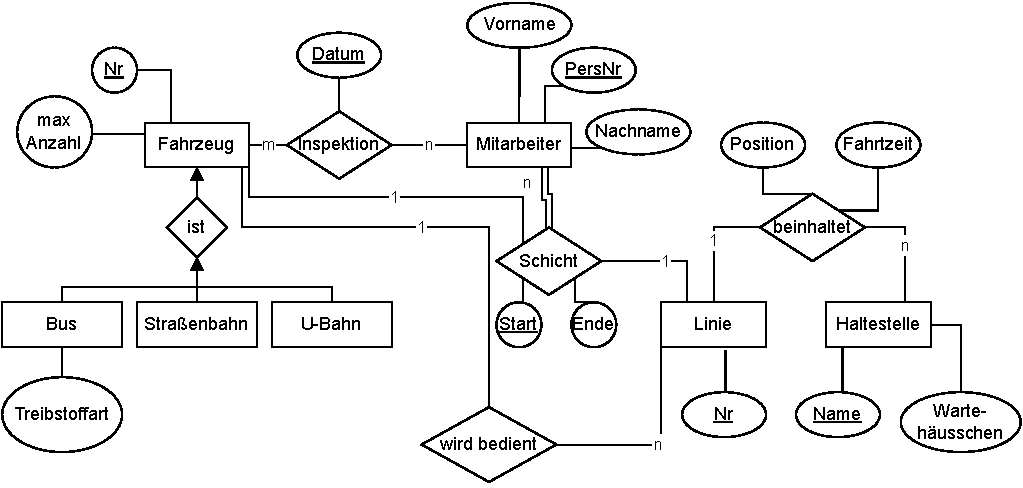
\includegraphics[scale=0.5]{F18Th1A2.pdf}
\end{figure}
	
\end{aufgabe}

\begin{aufgabe}%3
Agentur (\underline{Name}, E-Mail, Name_ü[Agentur]) \\
Person (\underline{PID}, \underline{Name}[Agentur], Nachname) \\
Kunde (\underline{PID}, \underline{Name}[Agentur], Geburtsdatum) \\
Berater (\underline{PID}, \underline{Name}[Agentur], Lohngruppe) \\
Vereinbarung (\underline{VID}, Bezeichung) \\
schließt (\underline{VID}[Vereinbarung], \underline{PID}[Kunde], \underline{Name}[Kunde], \underline{PID}[Berater], \underline{Name}[Berater], Datum) \\ %TODO Frage: Warum Name[Kunde], Kunde hat kein Attribut Name, nur totale Abhängigkeit zu Agentur.
Die 3NF (= 3. Normalform) ist für alle Relationen erfüllt, da jede Relation nur ein Attribut enthält, welches kein Primärschlüssel darstellt. Dadurch ist neben der als gegeben vorausgesetzte Atomarität der Werte jedes nicht zum Primärschlüssel gehörende Attribut voll von dem Primärschlüssel abhängig. Also ist die 2NF erfüllt. Außerdem hängt jedes Nichtschlüssel-Attribut ausschließlich vom Primärschlüssel funktional ab. Dies begründet sich erneut aus der Tatsache, dass nur ein Nichtschlüssel-Attribut in jeder Relation existiert. Dadurch ist auch die 3NF erfüllt. %TODO 3NF erfüllt da immer nur ein Nichtschlüssel-Attribut?
	
\end{aufgabe}

\begin{aufgabe}%4
	\begin{teile}
	%a
	\item
	\begin{sql}
	CREATE TABLE Buch
	(ISBN INTEGER PRIMARY KEY,
	Titel VARCHAR(50),
	ID INTEGER REFERENCES Autor (ID),
	Erscheinungsjahr INTEGER)
	\end{sql}
	%b 
	\item
	\begin{sql}
	CREATE TRIGGER NN
	AFTER INSERT OF Nachname ON Autor
	FOR EACH ROW
	WHEN (new Nachname IS NULL)
	BEGIN
	INSERT INTO Autor (new Nachname = 'NN)
	\end{sql}
	%c
	\item
	\begin{sql}
	SELECT Titel
	FROM Buch B, Autor A
	WHERE B.ID = A.ID
	AND Geburtsdatum < '01.01.1990'
	\end{sql}
	%d
	\item
	%e
	\item
	%f
	\item
	%g
	\item
	\begin{sql}
	grant(Vergabe)
	revoke(Entzug)
	\end{sql}
	\end{teile}
\end{aufgabe}

\begin{aufgabe}%5

\end{aufgabe}

\begin{aufgabe}%6
\begin{teile}
	\item 
	\item
\end{teile}
\end{aufgabe}

\begin{aufgabe}%7
 \begin{teile}
	\item Logische Optimierung transformiert relational Algebraausdrücke in äquivalente Ausdrücke, die zu schnellerem Ausführungsplan führen (Fokus: Ausgaben der einzelnen Operatoren werden möglichst klein), dazu werden z.B. Selektionen und Kreuzprodukte zu Joins zusammengefasst, die Reihenfolge der Joins optimiert und Selektionen und Projektionen möglichst früh durchgeführt. Die physische Optimierung baut auf die logische Optimierung auf und ermittelt für die jeweiligen logischen Operatoren einen möglichst guten physischen. Zudem wird entschieden, ob Indices benutzt werden können, Zwischenergebnisse materialisiert etc. Hier tatsächlicher Zugriff af Tabellen und Joins, theoretische Optimierung vs. praktische Algorithmenwahl, mathematische Operationen der Relationalen Algebra vs. ausführbare Algorithmen, die logischen Operator implementieren. 
	\item \mbox{}\\
	Achtung: Andere Notation mit griechischen Buchstaben empfohlen !\\
	\begin{tikzpicture}[->,>=stealth', semithick]
		\node (1) {PROJ( , (Kund.Vname, Kund.Nname))};
		\node[below =1] (4) {SEL( , Kund.ID=Rechng.Kund AND Rechng.Sum $>$ 500)};
		\node[below =4] (5) {CROSS(,)};
		\node[below left of =5] (6) {Kund};
		\node[below right of =5] (7) {Rechng};
		
		\path (7) edge node {} (5);
	\path (6) edge node {} (5);
	\path (5) edge node {} (4);
	\path (4) edge node {} (1);
	\end{tikzpicture}
	\item Join statt Kreuzprodukt (CROSS), Selektion (SEL) der Sum vorziehen vor Join
\end{teile}
\end{aufgabe}

\section{Teilaufgabe 2}
\setcounter{aufgcount}{0}

\begin{aufgabe}%1
	\begin{teile}
		\item 
		\item 
		\item 
		\item
	\end{teile}
\end{aufgabe}

\begin{aufgabe}%2
\begin{teile}
	\item 
	\item 
	\item 
\end{teile}
\end{aufgabe}

\begin{aufgabe}%3
\begin{teile}
	\item 
	\item 
	\item 
\end{teile}
\end{aufgabe}